\documentclass[10pt,a4paper]{article}
\usepackage[margin=2cm]{geometry}
\usepackage{amsmath,amssymb,booktabs,graphicx,caption,xcolor,float,hyperref,tikz}
\usetikzlibrary{arrows.meta,positioning,calc}
\hypersetup{colorlinks=true,linkcolor=blue!50!black,urlcolor=blue!50!black}
\captionsetup{font=small,labelfont=bf}
\title{\vspace{-1.2cm}\textbf{The value of the correct answer: a sham baseline}\\[2pt]
\large Simulation 2 (asynchronous activation), setup \texttt{task003-symmetric}}
\author{LLM-free simulator; report of 16 October 2026; runs of 15 October 2026\\
\small Measures of \texttt{blackboard\_efficiency\_info\_goal\_and\_resource\_handoff.md}, from the runs of the main report of the same date.}
\date{}
\begin{document}
\maketitle
\vspace{-1cm}

\paragraph{How the simulator works.} The world, \texttt{task\_003}, has three candidate allocations; A0 is the
correct one. Each of 24 agents is given one true fact and reasons as an exact Bayesian: its \emph{belief} is the
exact probability of A0, A1 and A2 given the facts it currently remembers. There are no rounds. Each agent acts
at random times, on average once per time unit: it reads $q$ posts drawn at random from the 48 most recent posts
on a shared \emph{board} (never its own), adds their facts to its memory, recomputes its belief, \emph{votes} by
probability matching (a vote drawn from its belief) and posts one remembered fact that supports its vote. Every
remembered fact is forgotten after a random lifetime (on average a fraction $\rho$ survives one time unit; reading
it again renews it). A \emph{controller} with a target, A0 (truth) or A2 (false), acts at random times at rate
$\lambda_c$ until $t = 30$: it reads $q_c$ recent agent posts and, unless the \emph{vote gate} (at least 75\% of
them from agents voting for its target) or the \emph{proof stop} (its target already proved) silences it, posts
the one fact from its pool that best supports its target, at most 30 messages per episode. Agents continue
alone until $t = 40$. Every episode is run three times with the same random draws: without a controller
(\emph{silent}), with the controller targeting A0 and with the one targeting A2.

\paragraph{The facts at the start.} All facts are true. The agents hold, together, a proof of A0; no single
agent does, and neither pool can prove its target (Table~\ref{tab:facts}).

\begin{table}[H]
\centering\small
\caption{Facts available at $t = 0$ and what each set implies, $P(\text{A0}, \text{A1}, \text{A2} \mid \text{facts})$.}
\label{tab:facts}
\begin{tabular}{lcc}
\toprule
set of facts & facts & $P(\text{A0}, \text{A1}, \text{A2})$ \\
\midrule
agents' facts, all together (24 agents, one fact each) & 18 distinct & (1, 0, 0): proves A0 \\
A0 pool (controller with target A0) & 12, of which 10 new to the agents & (0.963, 0.037, 0) \\
A2 pool (controller with target A2) & 12, of which 10 new to the agents & (0.114, 0, 0.886) \\
agents' facts + either pool & 28 distinct & (1, 0, 0) \\
\bottomrule
\end{tabular}
\end{table}

\paragraph{The runs.} Posts read by an agent $q \in \{3, 6, 12\}$; posts read by the controller
$q_c \in \{3, 6, 12, 24\}$; controller rate $\lambda_c \in \{0.5, 1, 2, 3, 4, 5, 6, 7, 8\}$ (one fact per
message); memory $\rho \in \{1, 0.75, 0.5, 0.25\}$; vote gate on and off; proof stop on; 1{,}000 episodes per
setting (1{,}740 settings). Unless stated otherwise: $q = 6$, $q_c = 12$, $\lambda_c = 1$ (the main setting,
which posts about as many facts as Simulation 1 with one fact per night), gate on. The vote gate is on throughout.


\paragraph{Summary.} We compare a controller that is given the correct answer (\emph{informed}) with a \emph{sham}
controller that intervenes in the same way but is given a target drawn at random, using the uncontrolled swarm as
the reference. \textbf{The paired correctness susceptibility $\chi_{\rm correct}$ and the two information numbers
$I(Z;X)$ and $I(Z;Y)$ behave like the susceptibility of the main report}: they grow as memory shortens
(Figures~\ref{fig:t075}--\ref{fig:t025}), reverse with the posts each agent reads (Figure~\ref{fig:prq}) and are
transient with full memory (Figure~\ref{fig:t1}). \textbf{The ratios $\eta_{\rm info}$ and $\eta_{\rm goal}$ do not
measure size}: across settings at $t = 30$, $\eta_{\rm info}$ is uncorrelated with $\chi_{\rm correct}$ (correlation
$-0.02$), and with full memory it climbs to 0.93--0.95 just as every effect fades to zero. \textbf{The per-fact return
$\eta_{\rm post}$ is the informative cost measure}: it falls steadily with the rate (0.05--0.06 to 0.014--0.018 per fact at
$t = 30$), and it rises with the posts the agents and the controller read because the informed controller then posts
fewer facts, not because the gain is larger.

\section{Quantities}\label{sec:quantities}

\paragraph{Treatment.} An episode-level treatment $Z$ is drawn with $P(Z = 1) = P(Z = 0) = 1/2$:
\begin{equation}\label{eq:Z}
Z = \begin{cases} 1, & \text{informed: the controller targets the correct answer, A0;}\\
0, & \text{sham: the controller's target is drawn by a fair coin from \{A0, A2\}, fixed for the episode.}\end{cases}
\end{equation}
The sham intervenes like the informed controller (same rate, budget, gate and reading) but is not given the correct
answer. This setup has pools for A0 and A2 only, so the sham draws from these two targets (the handoff suggests all
three answers; an A1 target would need a new pool). The sham coincides with the informed controller in half of its
episodes, by design. The \emph{uncontrolled} swarm (no controller) is the reference.

\paragraph{State and correctness.} $X_t$ is the vote of a randomly chosen agent at time $t$ (agents who have not
voted are left out); $Y_t = \mathbf 1\{X_t = \text{A0}\}$ says whether that vote is correct. With $x^{(e)}_{a,t}$ the
share of votes for $a$ in episode $e$,
\begin{equation}\label{eq:p}
p_{z,t}(x) = \mathbb E\bigl[x^{(e)}_{x,t}\,\big|\,Z = z\bigr], \qquad q_t(x) = \mathbb E^{0}\bigl[x^{(e)}_{x,t}\bigr],
\qquad \bar p_t = \tfrac12 p_{1,t} + \tfrac12 p_{0,t},
\end{equation}
where $\mathbb E^0$ is over uncontrolled episodes. The sham's distribution is exactly the average of the A0-target
and A2-target arms, $p_{0,t} = \frac12(p^{\rm A0}_t + p^{\rm A2}_t)$, because each arm's distribution is an average
over its episodes. Every episode was run in all three arms with the same random draws.

\paragraph{Paired correctness susceptibility and its return per fact.}
\begin{equation}\label{eq:chi}
\chi_{\rm correct}(t) = \mathbb E\bigl[m^{(e)}_{1}(t) - m^{(e)}_{0}(t)\bigr]
= \tfrac12\,\mathbb E\bigl[x^{(e),\rm A0}_{\text{A0},t} - x^{(e),\rm A2}_{\text{A0},t}\bigr],
\end{equation}
with $m^{(e)}_z$ the share of correct votes in episode $e$ under treatment $z$. In the notation of the main report it is
$\frac12(G^{+,0}_t - G^{-,0}_t)$, the directional half-contrast $D^{(0)}_t$: it adds the help of the informed
controller and the harm of the sham. With $F_t$ the facts posted by the informed controller up to $t$ (only its posts
are counted),
\begin{equation}\label{eq:post}
\eta_{\rm post}(t) = \chi_{\rm correct}(t)\,/\,\mathbb E[F_t],
\end{equation}
undefined below half a fact.

\paragraph{Information and the common cost.} With $\mathrm{KL}(p\Vert r) = \sum_x p(x)\log_2[p(x)/r(x)]$ (bits),
\begin{equation}\label{eq:C}
C_X(t) = \tfrac12\mathrm{KL}(p_{1,t}\Vert q_t) + \tfrac12\mathrm{KL}(p_{0,t}\Vert q_t)
= I(Z;X_t) + \mathrm{KL}(\bar p_t\Vert q_t),
\end{equation}
\begin{equation}\label{eq:info}
I(Z;X_t) = \tfrac12\mathrm{KL}(p_{1,t}\Vert\bar p_t) + \tfrac12\mathrm{KL}(p_{0,t}\Vert\bar p_t),\qquad
\eta_{\rm info}(t) = I(Z;X_t)/C_X(t),
\end{equation}
\begin{equation}\label{eq:goal}
I(Z;Y_t) = \tfrac12\mathrm{kl}(r_{1,t}\Vert\bar r_t) + \tfrac12\mathrm{kl}(r_{0,t}\Vert\bar r_t),\qquad
\eta_{\rm goal}(t) = I(Z;Y_t)/C_X(t),
\end{equation}
where $r_{z,t} = p_{z,t}(\text{A0})$, $\bar r_t = \bar p_t(\text{A0})$ and kl is the KL divergence between two-valued
distributions. $C_X$ is the change from no control caused by intervening at all; $I(Z;X)$ is the part of it that
depends on whether the controller had the correct answer; the rest, $\mathrm{KL}(\bar p\Vert q)$, does not. Because
$Y$ is computed from $X$,
\begin{equation}\label{eq:order}
0 \le I(Z;Y_t) \le I(Z;X_t) \le C_X(t), \qquad 0 \le \eta_{\rm goal} \le \eta_{\rm info} \le 1 .
\end{equation}
Both ratios are undefined when $C_X < 0.01$ bits. Every distribution gets the same pseudo-count of 0.5 episodes per
value before any KL, as in the main report. In the data, Eq.~(\ref{eq:C}) holds to $3\times10^{-16}$ bits and
Eq.~(\ref{eq:order}) holds everywhere. Neither information nor ratio has a sign: report them with $\chi_{\rm correct}$.

\paragraph{Relation to the main report.} There $Z$ was the controller's target (A0 against A2) and $C$ compared the
two targeted arms with silence. Here $Z$ is whether the target was the correct answer. The two information numbers
are closely related (correlation 0.98 across settings at $t = 30$), but the new ones are about a third as large,
because the sham shares half of its episodes with the informed controller.

\section{Observables as time series}\label{sec:time}

Each figure shows one memory $\rho$; top row: $\chi_{\rm correct}$ (bands: 95\% intervals; 0 at $t = 0$),
$\eta_{\rm post}$, $\eta_{\rm info}$, $\eta_{\rm goal}$; bottom row: $I(Z;X)$, $I(Z;Y)$ and $C_X$. One curve per
controller rate $\lambda_c$; $q = 6$, $q_c = 12$, gate on; the controller stops at $t = 30$ (dashed). Axes are the same
in all four figures.

\begin{figure}[H]
\centering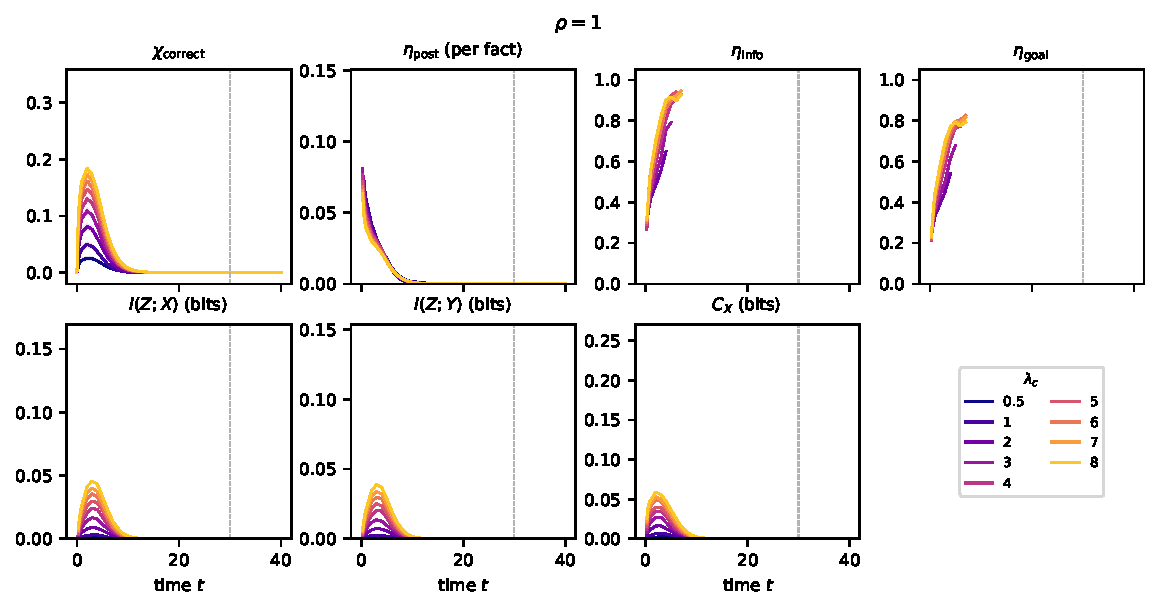
\includegraphics[width=0.95\linewidth]{figures/fig_time_rho1.pdf}
\caption{Full memory, $\rho = 1$. Blank: undefined ($C_X < 0.01$ bits, or under half a fact posted).}
\label{fig:t1}
\end{figure}

\begin{figure}[H]
\centering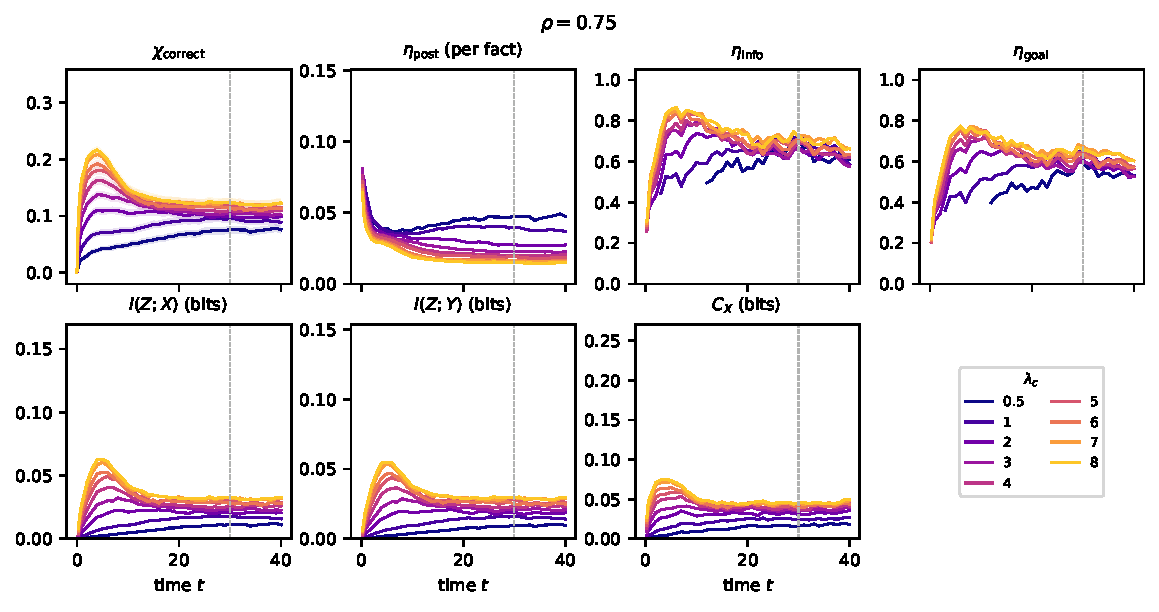
\includegraphics[width=0.95\linewidth]{figures/fig_time_rho0.75.pdf}
\caption{$\rho = 0.75$.}
\label{fig:t075}
\end{figure}

\begin{figure}[H]
\centering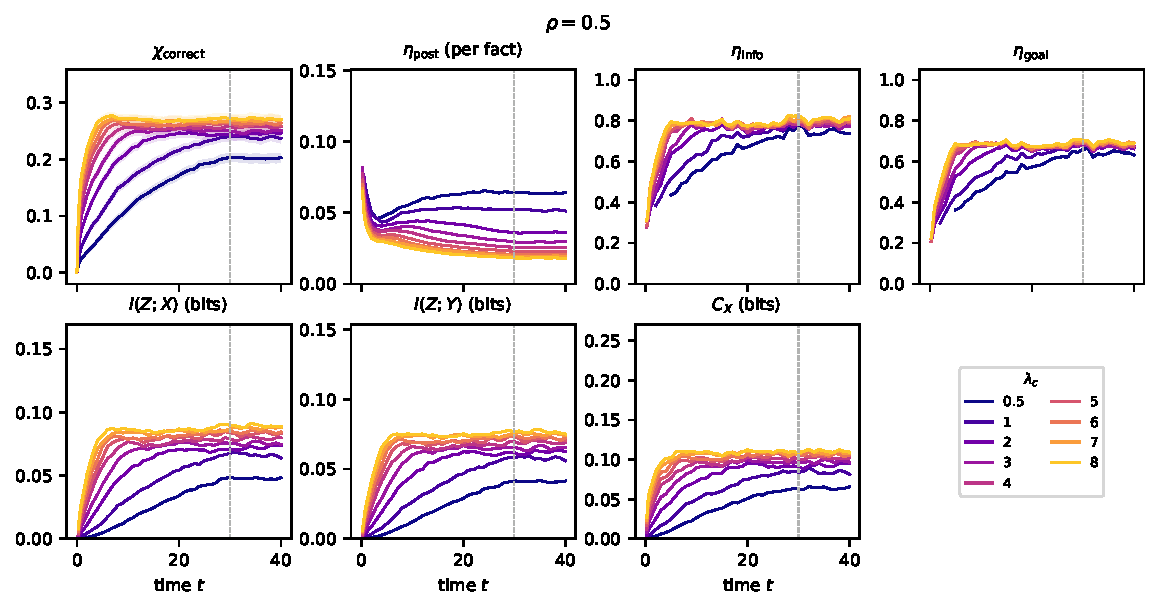
\includegraphics[width=0.95\linewidth]{figures/fig_time_rho0.5.pdf}
\caption{$\rho = 0.5$.}
\label{fig:t05}
\end{figure}

\begin{figure}[H]
\centering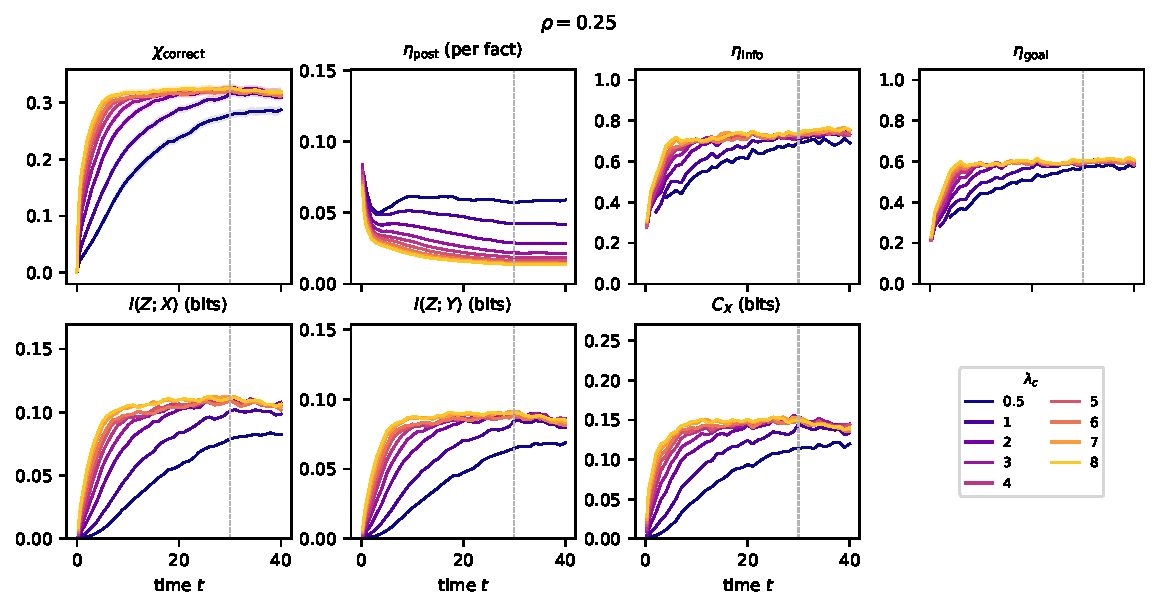
\includegraphics[width=0.95\linewidth]{figures/fig_time_rho0.25.pdf}
\caption{$\rho = 0.25$.}
\label{fig:t025}
\end{figure}

\begin{itemize}\itemsep1pt
\item \textbf{$\chi_{\rm correct}$ grows as memory shortens}: at $t = 30$, $0.08$--$0.12$ ($\rho = 0.75$),
  $0.20$--$0.27$ ($\rho = 0.5$), $0.28$--$0.33$ ($\rho = 0.25$), 0 with full memory, where it peaks at $0.18$
  ($t \approx 2$, $\lambda_c = 8$) and vanishes by $t \approx 10$.
\item \textbf{$I(Z;X)$, $I(Z;Y)$ and $C_X$ have the same shape as $\chi_{\rm correct}$}: they rise, overshoot where
  it overshoots, and persist after $t = 30$ ($I(Z;X) = 0.01$--$0.03$, $0.05$--$0.09$, $0.08$--$0.11$ bits at
  $t = 30$ for $\rho = 0.75, 0.5, 0.25$).
\item \textbf{Most of the information is about correctness}: $I(Z;Y)/I(Z;X) = 0.82$--$0.90$ at $t = 30$ for
  $\rho < 1$. The rest is in how the wrong votes split between A1 and A2.
\item \textbf{$\eta_{\rm info}$ and $\eta_{\rm goal}$ rise early and then flatten}: from $0.37$--$0.53$ and
  $0.29$--$0.44$ at $t = 1$ to $0.66$--$0.83$ and $0.57$--$0.70$ at $t = 30$, at every $\rho < 1$ and for every rate.
\item \textbf{With full memory the ratios climb as the effects vanish}: $\eta_{\rm info}$ reaches $0.93$--$0.95$ just
  before $C_X$ falls below $0.01$ bits (Figure~\ref{fig:t1}). A ratio of two vanishing numbers can be large; it says
  nothing about how much control there is.
\item \textbf{$\eta_{\rm post}$ falls with the rate and with time}: every controller starts near $0.04$--$0.07$ per
  fact; at $t = 30$ the slowest keeps $0.05$--$0.06$, the fastest $0.014$--$0.018$ (all $\rho < 1$).
\end{itemize}

\section{Phase diagrams}\label{sec:phase}

All panels at $t = 30$, gate on; colour scales are shared by the three figures. Grey number in $\chi_{\rm correct}$:
its 95\% interval includes 0. Dash: undefined.

\begin{figure}[H]
\centering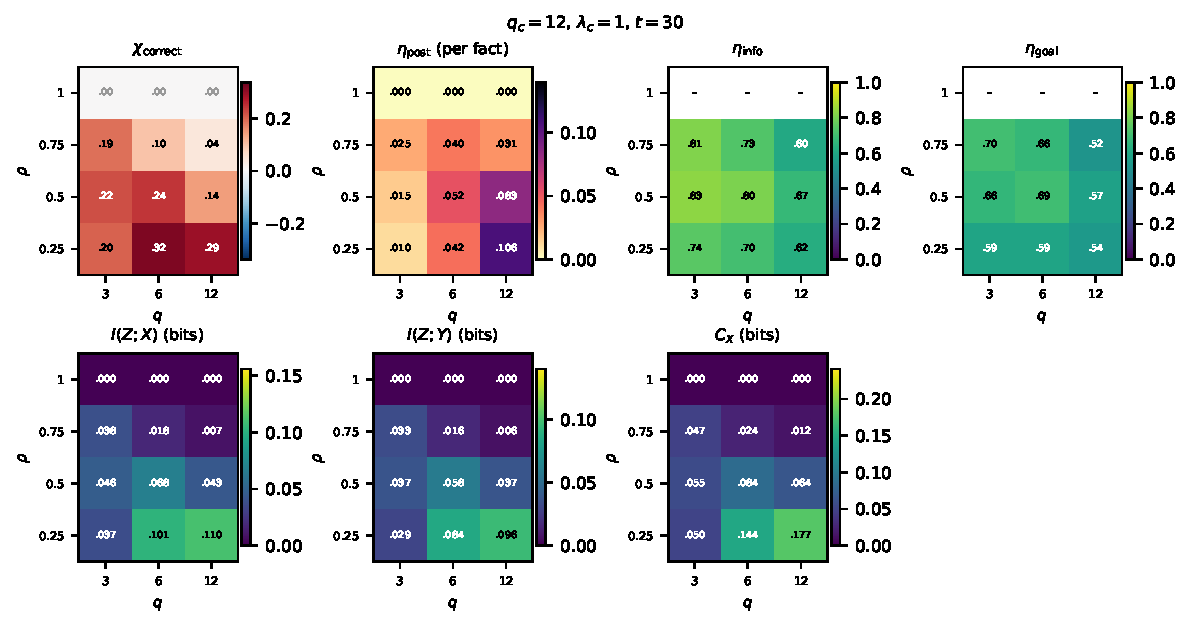
\includegraphics[width=0.98\linewidth]{figures/fig_phase_rho_q.pdf}
\caption{Over memory $\rho$ and the posts each agent reads $q$; $q_c = 12$, $\lambda_c = 1$.}
\label{fig:prq}
\end{figure}

\begin{itemize}\itemsep1pt
\item \textbf{The reversal with $q$ is in $\chi_{\rm correct}$ and the information numbers}: at $\rho = 0.75$,
  $\chi_{\rm correct}$ falls from $0.19$ ($q = 3$) to $0.04$ ($q = 12$) and $I(Z;X)$ from $0.038$ to $0.007$ bits; at
  $\rho = 0.25$ they rise from $0.20$ to $0.29$--$0.32$ and from $0.037$ to $0.10$--$0.11$.
\item \textbf{$\eta_{\rm info}$ and $\eta_{\rm goal}$ do not show it}: they fall with $q$ at every $\rho$
  ($\eta_{\rm info}$ $0.81 \to 0.60$ at $\rho = 0.75$; $0.74 \to 0.62$ at $\rho = 0.25$).
\item \textbf{$\eta_{\rm post}$ rises with $q$} ($0.010 \to 0.106$ per fact at $\rho = 0.25$) because the informed
  controller posts fewer facts when agents read more (19 against 3 by $t = 30$), likely because its gate finds
  agreement sooner (not checked).
\end{itemize}

\begin{figure}[H]
\centering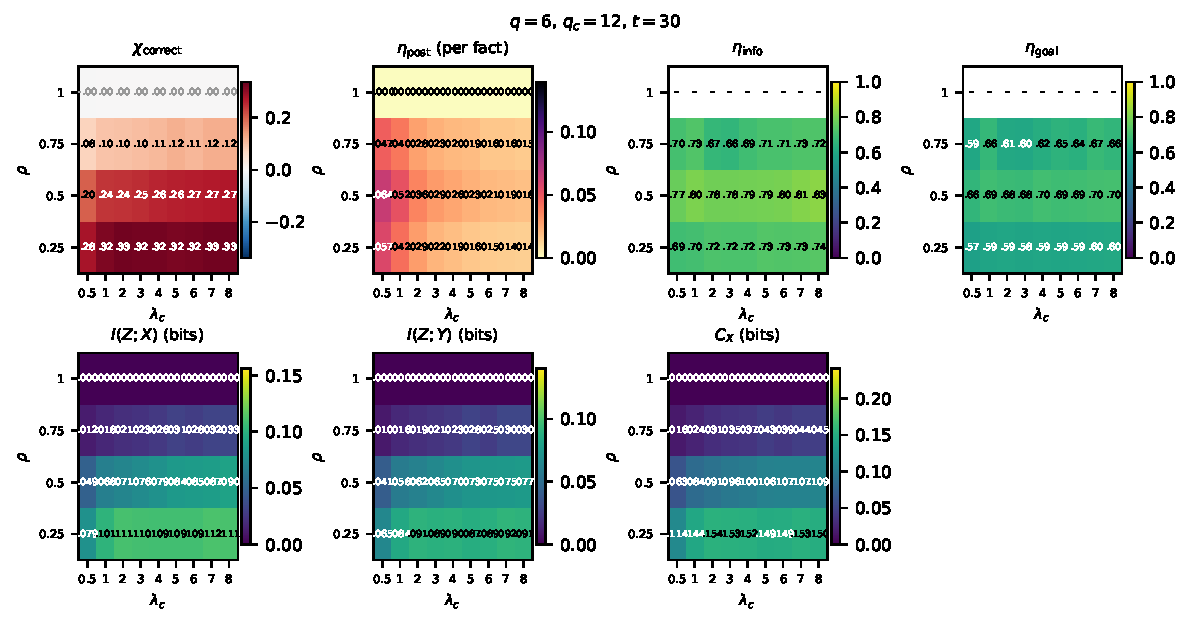
\includegraphics[width=0.98\linewidth]{figures/fig_phase_rho_x.pdf}
\caption{Over memory $\rho$ and the controller rate $\lambda_c$; $q = 6$, $q_c = 12$.}
\label{fig:prx}
\end{figure}

\begin{itemize}\itemsep1pt
\item \textbf{Memory sets $\chi_{\rm correct}$, $I(Z;X)$, $I(Z;Y)$ and $C_X$; the rate barely does}: along each row
  they change little beyond $\lambda_c = 1$, as the main report's susceptibility does.
\item \textbf{$\eta_{\rm info}$ and $\eta_{\rm goal}$ stay at $0.66$--$0.83$ and $0.57$--$0.71$} over the whole
  diagram, highest at $\rho = 0.5$, with no relation to the size of $\chi_{\rm correct}$.
\item \textbf{$\eta_{\rm post}$ falls along every row}, from $0.05$--$0.06$ at $\lambda_c = 0.5$ to $0.014$--$0.018$
  at $\lambda_c = 8$: faster control adds facts but little correctness.
\end{itemize}

\begin{figure}[H]
\centering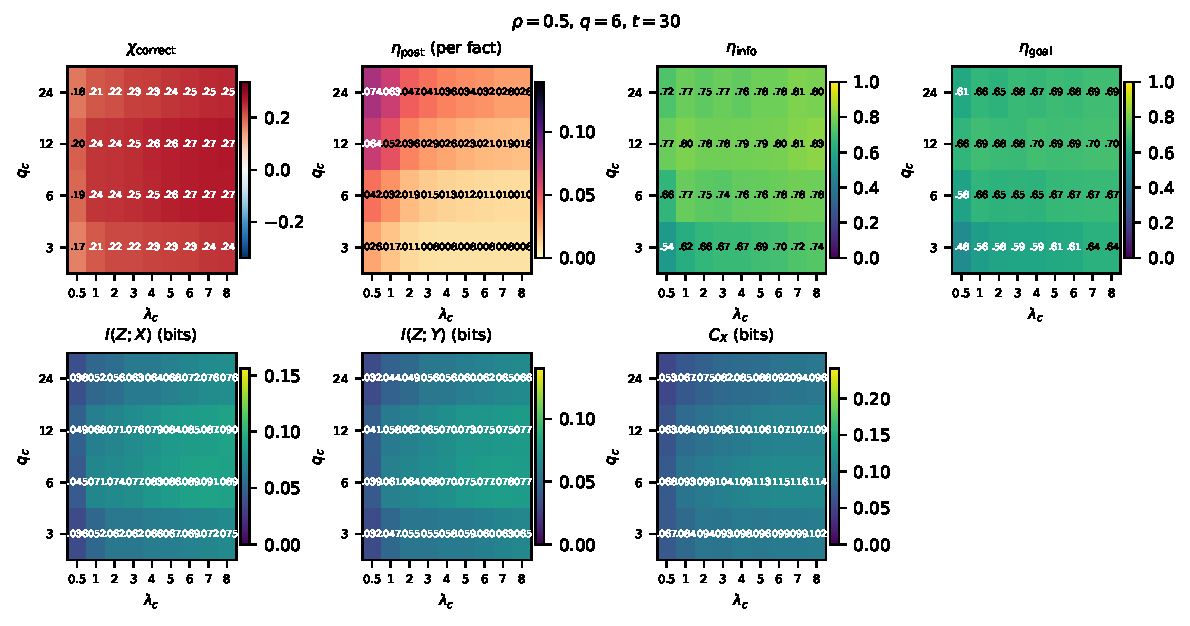
\includegraphics[width=0.98\linewidth]{figures/fig_phase_qc_x.pdf}
\caption{Over the posts the controller reads $q_c$ and its rate $\lambda_c$; $\rho = 0.5$, $q = 6$.}
\label{fig:pqx}
\end{figure}

\begin{itemize}\itemsep1pt
\item \textbf{The controller's reading hardly changes $\chi_{\rm correct}$} (mean $0.22$, $0.25$, $0.25$, $0.23$ for
  $q_c = 3, 6, 12, 24$) \textbf{but quadruples $\eta_{\rm post}$} ($0.011 \to 0.043$ per fact), because it posts fewer facts (24 at $q_c = 3$, 6 at
  $q_c = 24$, by $t = 30$), likely because reading more lets its gate stop it sooner (not checked).
\item \textbf{$\eta_{\rm info}$ and $\eta_{\rm goal}$ rise slightly with $q_c$} ($0.67 \to 0.77$--$0.80$ and
  $0.59 \to 0.67$--$0.69$).
\end{itemize}

\section{Conclusions}

\begin{enumerate}\itemsep2pt
\item \textbf{The sham baseline gives a clean signed measure}: $\chi_{\rm correct}$ follows the size of control as the
  main report's susceptibility does (correlation with $I(Z;X)$ across settings: 0.90). It mixes the informed
  controller's help with the sham's harm, so it should be read next to the gain against no control.
\item \textbf{$\eta_{\rm info}$ and $\eta_{\rm goal}$ are not efficiencies of control.} Across settings they are
  uncorrelated with $\chi_{\rm correct}$ ($-0.02$), they hide the reversal with $q$, and they approach 1 as every
  effect vanishes. Their numerators and $C_X$ carry the information; the ratios describe only how the change is
  split, as the handoff warns.
\item \textbf{$\eta_{\rm post}$ is the useful cost measure}, with one caution: it rises whenever the informed
  controller posts less, so a setting that silences the controller sooner (more reading by agents or controller)
  looks more efficient per fact even when $\chi_{\rm correct}$ does not change.
\item \textbf{Most target information is about correctness} ($I(Z;Y)/I(Z;X) = 0.82$--$0.90$).
\end{enumerate}

\paragraph{Caveats.} Simulation 2, \texttt{task003-symmetric}, one world; a sham over the two targets that have
pools; 1{,}000 episodes per arm. Reads are not charged: the handoff's $\eta_{\rm ops}$ would add them with a weight
fixed in advance. Data: \texttt{results/simulation\_2/2026-10-15\_sim2\_symmetric\_fine}; table:
\texttt{results/gold\_standard/2026-10-15/sham\_table.parquet}; code: \texttt{analysis/task003\_llm\_free/shared\_analysis/gold\_standard/sham\_baseline*.py}.

\end{document}
